\documentclass[ignorenonframetext, professionalfonts, hyperref={pdftex, unicode}]{beamer}
%\usepackage{beamerthemesplit}

\geometry{paperwidth=140mm,paperheight=105mm}

%Hack to specify beamer folder https://tex.stackexchange.com/questions/275600/beamer-themes-on-custom-folder
\makeatletter
  \def\beamer@calltheme#1#2#3{%
    \def\beamer@themelist{#2}
    \@for\beamer@themename:=\beamer@themelist\do
    {\usepackage[{#1}]{\beamer@themelocation/#3\beamer@themename}}}

  \def\usefolder#1{
    \def\beamer@themelocation{#1}
  }
  \def\beamer@themelocation{}
\makeatother
%Packages to be included

\usepackage{graphicx}



\graphicspath{{./branding/}}
\usefolder{./branding}
\usetheme{Promwad}
%\usecolortheme{wolverine}


\usepackage[russian]{babel}
\usepackage[utf8]{inputenc}
\usepackage[T1]{fontenc}

%\usepackage[orientation=landscape, size=custom, width=16, height=9, scale=0.5]{beamerposter}

\usepackage{textcomp}


\usepackage{ulem}

\usepackage{verbatim}

\usepackage{ucs}


\usepackage{listings}
\lstloadlanguages{bash}

\lstset{escapechar=`,
	extendedchars=false,
	language=sh,
	frame=single,
	tabsize=2, 
	columns=fullflexible, 
%	basicstyle=\scriptsize,
	keywordstyle=\color{blue}, 
	commentstyle=\itshape\color{brown},
%	identifierstyle=\ttfamily, 
	stringstyle=\mdseries\color{green}, 
	showstringspaces=false, 
	numbers=none, 
%	numberstyle=\tiny, 
	breaklines=true, 
	inputencoding=utf8,
	keepspaces=true,
	morekeywords={u\_short, u\_char, u\_long, in\_addr}
	}

\definecolor{darkgreen}{cmyk}{0.7, 0, 1, 0.5}

\lstdefinelanguage{diff}
{
    morekeywords={+, -},
    sensitive=false,
    morecomment=[l]{//},
    morecomment=[s]{/*}{*/},
    morecomment=[l][\color{darkgreen}]{+},
    morecomment=[l][\color{red}]{-},
    morestring=[b]",
}

\author[Promwad]{{\bf Promwad}}

%\institution[EPAM]{EPAM}
%\logo{\includegraphics[width=1cm]{logo.png}}

\AtBeginSection[]{%
  \begin{frame}<beamer>
    \frametitle{}
    \tableofcontents[
        sectionstyle=show/shaded, hideallsubsections ]
  \end{frame}
  \addtocounter{framenumber}{-1}% If you don't want them to affect the slide number
}

\AtBeginSubsection[]{%
  \begin{frame}<beamer>
    \frametitle{}
    \tableofcontents[
        sectionstyle=show/hide,
        subsectionstyle=show/shaded/hide, ]
  \end{frame}
  \addtocounter{framenumber}{-1}% If you don't want them to affect the slide number
}


% Comment to disable notes 
\usepackage{./branding/notes}


\AtBeginSection[]{
  \begin{frame}
  \vfill
  \centering
  \begin{beamercolorbox}[sep=8pt,center,shadow=true,rounded=true]{title}
    \usebeamerfont{title}\insertsectionhead\par%
  \end{beamercolorbox}
  \vfill
  \end{frame}
}

\begin{document}


\begin{titlepage}
\title{Встраиваемые системы. Введение}
\end{titlepage}

%%%%%%%%%%%%%%% Особенности %%%%%%%%%%%%%%%%%%
\section{Понятие <<Встраиваемые системы>>. Особенности}

\begin{frame}[fragile]{Понятие <<Встраиваемые системы>>}
\begin{itemize}
	\item \textcolor{blue}{Встраиваемая система} - общее понятие, которым можно охарактеризовать все устройства, которые не относятся к компьютерам общего назначения.
	\item \textcolor{blue}{Встраиваемая система} – это система, у которой имеется тесная связь между аппаратным и программным обеспечением. В большинстве случаев ПО нельзя рассматривать в отрыве от аппаратного обеспечения, конструкции и особенностей окружения.
	\item \textcolor{blue}{Встраиваемые системы} – это всегда специализированные системы.
\end{itemize}

\note{\begin{itemize}
\item Можно найти серию определений.
Связано это с тем, что за период эволюции грань между встраиваемыми системами и компьютерами общего назначения сильно размылась.
\item Так например, если взять современный смартфон. То с одной стороны его аппаратную начинку можно больше отнести к встраиваемым системам.
В тоже время по использовании программной части и предоставляемой возможности расширять функциональность за счет установки дополнительного программного обеспечения – больше относится к компьютерам общего назначения.
\item Кроме того ВС имеют градацию в зависимости от области применения - офисное оборудование, коммуникационные системы, медицинское оборудование.
\item И в зависимости от области применения могут предъявляться разные требования. Такие как требования к надежности,  требования обработки событий в режиме реального времени, либо даже требования к аппаратным ресурсам с целью минимизации стоимости. и так далее.
\end{itemize}
} %note
\end{frame}

\begin{frame}[fragile]{IP-камера как пример ВС}
\begin{center}
 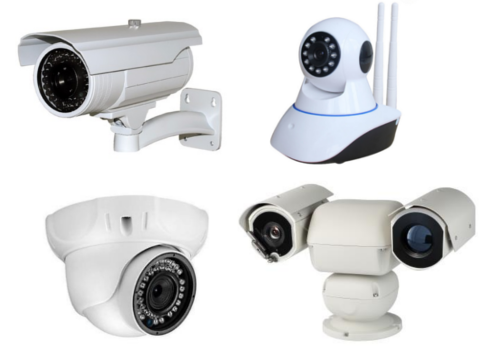
\includegraphics[width=8cm]{ip-camera_samples.png}
\end{center}
\note{
Уверен, что если я попрошу вас привести пример ВС - вы с легкостью приведете. Каждый встречал ВС. Кто-то вспомнит:
  \begin{itemize}
  \item про плеер в своем кармане или цифровой фотоаппарат.
  \item про цифровые табло расписания на автобусной остановке.
  \item про микроволновую печь на кухне
  \item про доильные аппараты на своем предыдущем месте работы... 
  \end{itemize}
И вы будете абсолютно правы.\\
Я бы хотел привести пример IP-камеры. Как отличный пример встраиваемой системы на базе GNU/Linux. И мало того, я предлагаю в рамках этих лекций ввести вымышленный проект IP-камеры под кодовым словом <<ОКО>>. B для этой камеры нам якобы предстоит разработать прошивку. Мне кажется, что это даст возможность:
  \begin{itemize}
  \item Мне будет проще пояснять вам теоретические аспекты, приводя примеры из конкретного проекта.
  \item Вы параллельно сможете отследить основные этапы разработки встраиваемой систем на базе GNU/Linux. И, возможно, это поспособствует более качественному закреплению материалов.
  \end{itemize}
\\
Поэтому давайте сразу представим себя командой матерых embedded-разработчиков, которым предстоит разработать прошивку для IP-камеры. И обладать она будет вполне себе тривиальными возможностями. \\

} %note
\end{frame}


\begin{frame}[fragile]{Проект "ОКО"}
 \textcolor{blue}{IP-видеокамера}. Возможности устройства:
 \begin{itemize}
  \item Захватывать данные с камеры и микрофона
  \item Кодировать видеоданные:
  	\begin{itemize}
  	\item Видео в H.264, MJPEG;
  	\item Aудио в VOIP-совместимый формат 
	 \end{itemize}  	 
  \item Транслировать медиаданные по сети:
   	\begin{itemize}
  	\item RTP/RTSP - видео, аудио;
  	\item over HTTP - видео в формате MJPEG
	 \end{itemize}  	 
 \end{itemize}		  
\note{
Давайте сразу очертим возможности нашей камеры. Своего рода составим техническое задание.\\
Прежде всего камера будет выполнять свою основную задачу. Делать захват медиаданных и транслировать в сеть клиенту. При этом все будет стандартно для того рода устройств. Кодеки будут общепринятые и способы трансляции.\\

} %note
\end{frame}


\begin{frame}[fragile]{Проект <<ОКО>>}
 \textcolor{blue}{IP-видеокамера}. Возможности устройства:
 \begin{itemize}
  \item Поддержка тревожные события:
  	\begin{itemize}
  	\item Детектор движения
  	\item Аудио детектор
  	\item Изменение состояния геркона
	 \end{itemize}  	 
  \item Реакция на тревожные события 
   	\begin{itemize}
  	\item Запись на карту памяти медиаданных
  	\item Регистрация события в логах
	\end{itemize}  	 	
 \end{itemize}		
  
\note{
Для того, чтобы проект не был уж совсем примитивным реализуем в нем поддержку тревожных событий. Мы будем их детектировать и производить реакцию. Как минимум будем оставлять строчку в логах работы и производить запись видео- аудио-обстановки на карту памяти. Возможно мы еще захотим оповещать через telegram-бота. Но поддержка таких возможностей особо не повлияет на сложность проекта.\\

} %note
\end{frame}

\begin{frame}[fragile]{Проект <<ОКО>>}
 \textcolor{blue}{IP-видеокамера}. Возможности устройства:
 \begin{itemize}
  \item Управление устройством:
   	\begin{itemize}
  	\item Веб-интерфейс
  	\item CLI-интерфейс с доступом по SSH.
  	\item ONVIF
	\end{itemize}
  \item Дополнительные возможности:
   	\begin{itemize}
  	\item Управление поворотным устройством
  	\item Управление ИК-подсветкой камеры
  	\item Замыкать сухой контакт
	\end{itemize}  	   	 
 \end{itemize}		
  
\note{
Ну и еще несколько возможностей я бы хотел добавить. Которые мне позволят изложить более качественно материал лекций.\\
Прежде всего, мы хотим сделать поддержку управления устройством. Веб-интерфейс по сути будет являться основным клиентом по настройке устройства. \\
CLI-интерфейс скорее больше нужен как диагностическая утилита, либо как средство по быстрому изменению настроек. \\
ONVIF - это ряд спецификаций, который позволяет наладить обмен с другими устройствами из области систем наблюдения. При этом устройства могут быть разных производителей. В нашем случае можно рассмотреть ситуацию, когда к нашей камере может подключиться ONVIF-клиент стороннего разработчика. И управлять ей в обход веб-интерфейса или CLI. При этом это будет выглядеть как будто это наш родной клиент.\\
Возможно, в следующих лекциях я более подробно затрону ONVIF с точки зрения реализации. \\
Сделаем также поддержку управления инфракрасной подсветкой в ночное время. И также будем еще управлять областью обзора камеры с помощью поворотного устройства, на котором она и будет закреплена.\\\\
Ну и наша камера еще сможет управлять реле, с помощью котором мы, например, сможем блокировать/отпирать входную дверь. Или еще что, где подразумевается операция <<включить>>/<<выключить>>

} %note
\end{frame}



\begin{frame}[fragile]{Встраиваемые системы. Специфика}
По сравнению с компьютерами общего назначения \textcolor{blue}{шире ряд используемых процессоров}:
\begin{itemize}
	\item ARM
	\item PowerPC
	\item MIPS
	\item Blackfin
	\item x86, x86/64
\end{itemize}

\note{
Если начать рассматривать особенности ВС по сравнению с компьютерами общего назначения можно сразу выделить то, что гораздо шире ряд  процессоров. и x86 x64 занимают очень малую нишу.\\
} %note
\end{frame}


\begin{frame}[fragile]{Встраиваемые системы. Специфика}
\textcolor{blue}{Операционная система:}
\begin{itemize}
	\item Отсутствует  (Bare-metal) - ОС как таково отсутствует
	\item ОС реального времени, например FreeRTOS
	\item ОС GNU/Linux, Windows CE, Android	
\end{itemize}
\note{
С точки зрения наличия операционной системы можно выделить варианты когда операционная система отсутствует.  Либо запущена ОС реального времени. Либо запущена встраиваемая ОС. \\
Не всегда это связано с ресурсами нашего устройства. \\
Например вполне себе может быть ситуация, когда в рамках одного устройства выполняются две системы - система реального времени (для выполнения критичных задач) и Linux (для выполнения рутинных задач, не требующих real-time).\\

} %note
\end{frame}

\begin{frame}[fragile]{Встраиваемые системы. Специфика}
\begin{itemize}
\item \textcolor{blue}{Шире интерфейсы взаимодействия}
\begin{itemize}
	\item кейпады, IR-приемники
	\item Символьные дисплеи, Светодиодная индикация
	\item и т.д
\end{itemize}
\item  Функциональные возможности системы могут иметь как \textcolor{blue}{аппаратную} так и \textcolor{blue}{программную} реализацию.
\\
\item \textcolor{blue}{Ресурсы могут быть ограничены}
\item Актуально \textcolor{blue}{внезапное отключение питания}
\end{itemize}
\note{\begin{itemize}
\item Если рассматривать компьютеры общего назначения, то можно выделить клавиатуры, экран, тач-панель мышь.
\item В тоже время можно рассмотреть ситуацию когда во встраиваемой системе:
\\ - одна и та же кнопка с точки зрения варианта взаимодействия может выполнять разные функции (ShortPress / LongPress)
\\ - вместо экрана для визуализации может быть только один светодиод. И то с какой частотой он моргает или просто горит - доноситься информация о состоянии системы.  
\item  Аппаратная/Программная реализация - задача может быть решена как аппаратно, так и программно. Убедимся далее по лекции
\item Следует также принимать во внимание, что диапазон рабочих температур ВС  может быть более суров, чем у компьютеров общего назначения. И можно также выделить и то, что во встраиваемых системах чаще приходится иметь дело с ситуацией <<Внезапная потеря питания>>. И нужно быть к этому готовым, в плане сохранения данных.
\end{itemize}
} %note
\end{frame}

\begin{frame}[fragile]{Встраиваемые системы. Специфика}
\textcolor{blue}{SoC - (System on Chip,система на кристалле)} -  наиболее часто используемое решение для встраиваемых систем на базе Linux\\

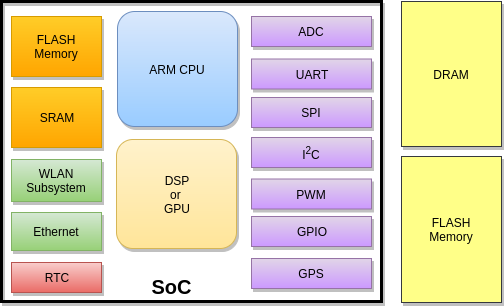
\includegraphics[width=8cm]{soc.png}
\note{
В большинстве случаев вам придется иметь дело с SoC-системами. SoC подразумевает, что в одну интегральную схему вмещается электронная схема, выполняющая функции целого устройства. На рисунке представлен абстрактный SoC, где для примера показаны возможные функциональные блоки в которые в него могут входить. \\
И по сути получается, что задействовав подобный SoC в проекте, нам достаточно сделать минимальную <<обвязку>>. С точки зрения схемы электрической принципиальной.  Например реализовать схему питания, добавить антенну и т.д. \\
Единственно что обычно используют совместно с SoC в виде отдельных компонент схемы - это память. Согласитесь, так проще варьировать размерами доступной оперативной памяти устройства, или энергонезависимой памяти. Но в то же время в SoC может присутствовать и своя память, но ее объемы обычно не исчисляются десятками мегабайт. Это могут быть килобайты. \\
\textcolor{blue}{SoC могут быть как универсальные, так и явно заточенные под определенную область применения}.\\

} %note
\end{frame}



%%%%%%%%%%%%%%% Общие определения %%%%%%%%%%%%%%%%%%
\section{Термины и понятия}

\begin{frame}[fragile]{Хост-машина}

\textcolor{blue}{Host development system (workstation)} - инструментальная машина, на которой идет процесс разработки программного обеспечения (далее хост-машина, хост).
 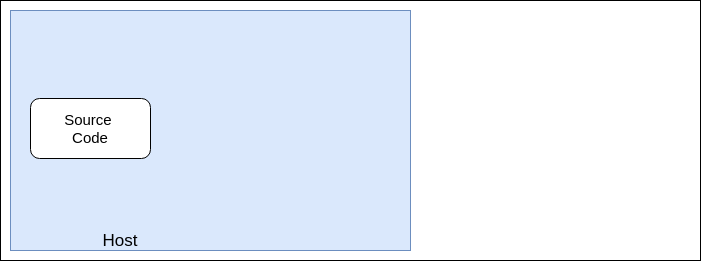
\includegraphics[width=8cm]{intro_host_target001.png}
\note{Рассмотрим с вами ряд понятий, которые будем использовать. Прежде всего, машина, на которой идет процесс разработки программного обеспечения, называется хост-машина. \\
В  большинстве случае под этой машиной подразумеваться компьютер общего назначения.\\
} %note
\end{frame}

\begin{frame}[fragile]{Набор инструментов}
\textcolor{blue}{GNU Toolchain} - набор пакета программ, необходимых для компиляции и генерации выполняемого кода из исходных текстов (далее "набор инструментов", тулчейны)
 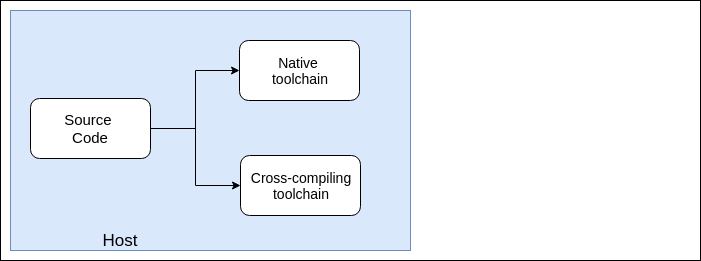
\includegraphics[width=8cm]{intro_host_target002.png}
\note{
Тулчейны могут быть нативными, то есть позволяют собирать программы для той же платформы что и хост-машина. И в таком случае разработанное приложение может быть запущено как на хост-машине, так и на устройстве. \\
Но могут быть тулчейны, которые позволяют собирать программы для других платформ. И в таком случае собранное приложение может быть запущено только на устройстве с архитектурой, для которой оно собиралось. \\
Такие наборы инструментов называют <<наборы инструментов кросс-сборки>>. И процесс компиляции программ называют кросс-компиляцией.\\
} %note
\end{frame}

\begin{frame}[fragile]{Целевая машина}
\textcolor{blue}{Target system} - целевая платформа, для которой разрабатывается программное обеспечение (далее целевое устройство, Target)
 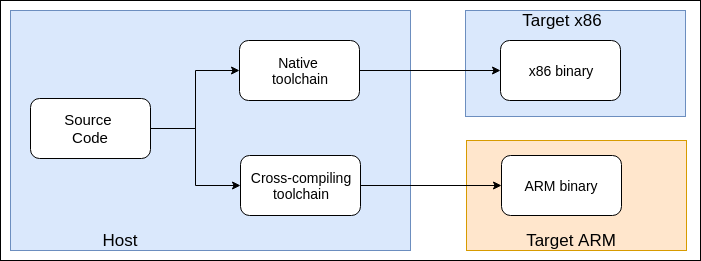
\includegraphics[width=8cm]{intro_host_target003.png}
\note{
Программное обеспечение разрабатывается для целевого устройства. Бывают случаи, когда, с точки зрения терминов, целевое устройство может выступать и хост-машиной. Например  Raspberry PI3 (далее RPI3) имеет достаточные ресурсы и объемы памяти, чтобы на ней самой установить средства сборки и на ней же писать код программы и собирать. Но обычно это частные случаи. \\

} %note
\end{frame}

\begin{frame}[fragile]{Встраиваемая операционная система}
\textcolor{blue}{Embedded OS} - операционная система, которая портирована и запускается на целевой платформе 
\linebreak
Является <<обезжиренной>> версией Linux:
\begin{itemize}
\item Поддержка железа на уровне ядра только для Target-платформы;
\item Софт используется только необходимый. Удаляются Man-ы и другие менее значимые ресурсы.
\item Используются более легковесные версии Веб-серверов, SSH, СУБД и т.д.
\end{itemize}

\note{\begin{itemize}
\item Если мы говорим о встраиваемой операционной системе в контексте Linux - мы имеем ввиду <<обезжиренный>> дистрибутив Linux, в который включено только самое необходимое программное обеспечение. 
\end{itemize}
} %note
\end{frame}

\begin{frame}[fragile]{Отладочные платы}
Development board выпускаются производителям SoC-систем. Cодержат:
\begin{itemize}
	\item Сам SoC
	\item Периферийная <<обвязка>> - для тестов возможностей SoC 
	\item Средства отладки. Позволяют зашить прошивку и отслеживать ее выполнение
\end{itemize}
\note{\begin{itemize}
\item Производители систем на кристалле выпускают макетные отладочные платы. Которые позволяют оценить возможности чипа. Либо начать разработку.
\item Обычно отладочные платы являются отправной точкой в проекте. Когда мы еще не имеем платы устройства-продукта, но можем уже начинать разрабатывать программное обеспечение для проекта
\end{itemize}
} %note
\end{frame}

\begin{frame}[fragile]{Примеры отладочных плат}
Пример обычной отладочной платы. \\
Qualcomm Mobile Hardware Development Kit 
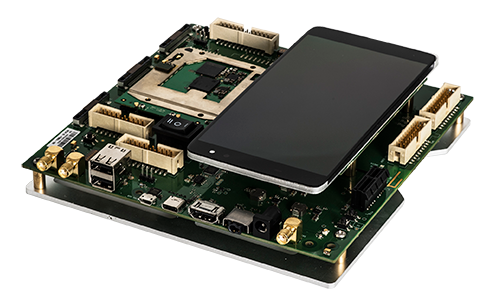
\includegraphics[width=8cm]{qualcomm-board.png}
\note{
Отладочные платы могут представлять собой обычную плату вне корпуса. Либо даже отдаленно напоминать устройство. В качестве случайно взятого примера можно рассмотреть DevKit производителя Qualcomm. Которая предназначена для разработки мобильного устройства.\\

} %note
\end{frame}

\begin{frame}[fragile]{Примеры отладочных плат}
Qualcomm Mobile Hardware Development Kit 
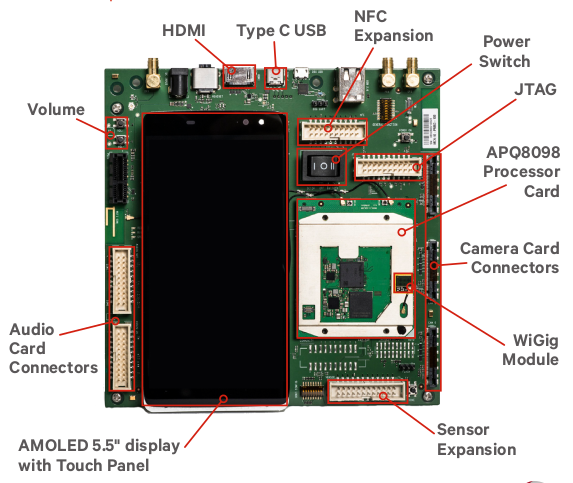
\includegraphics[width=7.5cm]{qualcomm-board2.png}
\note{
Как вы можете видеть на плате выполнена обвязка, которая позволяет инженеру с одной стороны легко подключить для тестов периферию. С другой стороны есть возможность получить доступ для снятия оцилограмм, расширить плату другими модулями и т.д. И как вы понимаете такая плата по окончанию проекта уже не нужна.  Обычно стоят платы от нескольких сотен, до нескольких тысяч долларов.

} %note
\end{frame}


\begin{frame}[fragile]{Примеры отладочных плат}
Дешевые макетные платы.
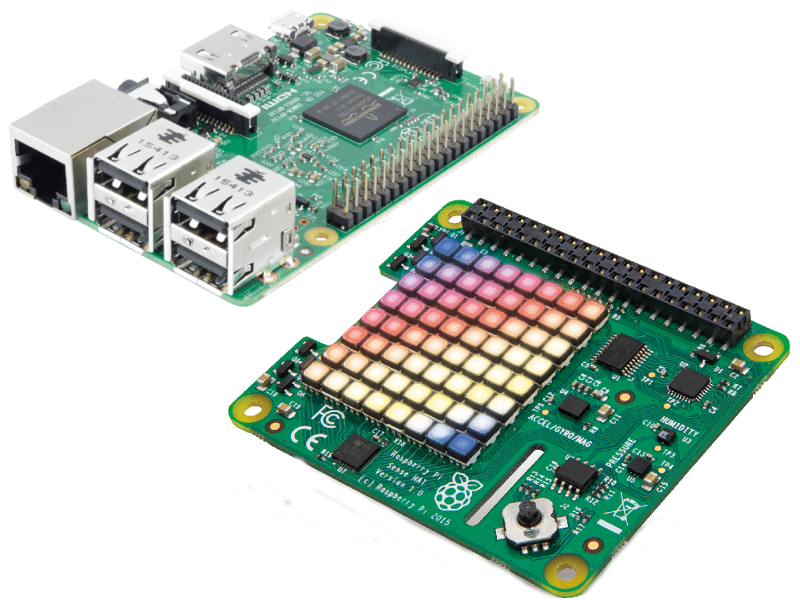
\includegraphics[width=8cm]{rpi_shield.png}
\note{
Отдельным, важным классом можно выделить целый ряд дешевых макетных плат. С доступной ценой для рядового пользователя. Который может использовать в хобби-проектах. 
Arduino, BeagleBoard/BeagleBone, Raspberry PI и их клоны. Такие платы как раз в первую очередь рассчитаны на хобби. И вокруг таких плат развились целые экосистемы. Которые имеют даже свою специфику. Так, например, если вы заинтересуетесь проектами под RPI3, то отметите для себя, что большинство проектов реализуется на языке Python. Полно примеров как работать с камерой, подключенными светодиодами и т. д. Но сам язык Python - не специфичен для эмбеддинга. Но его низкий порог вхождения позволяет любителю сравнительно легко добиться ожидаемого результата. \\
С другой стороны для этих плат начали появляться кастомные шилды от других производителей. Которые расширяют возможности этих плат. Так на рисунке, помимо платы RPI3, случайным образом выбран шилд, который имеет:
\begin{itemize}
	\item LED-дисплей 8x8
	\item гироскоп
	\item датчик температуры
	\item джойстик
\end{itemize}
Купив который можно приобрести опыт работы с подобной периферией. \\
Возвращаясь к самим платам с уверенностью можно сказать, что они могут быть рассмотрены и как полноценные решения для коммерческих проектов. Когда нет возможности или желания разрабатывать свое устройство. И по характеристикам они подходят для проекта\\
} %note
\end{frame}

\begin{frame}[fragile]{SDK,BSP}
Производители SoC, Отладочных плат предоставляют конечному пользователю
\begin{itemize}
	\item Board Support Package (BSP) - набор драйверов/модулей операционной системы для поддержки чипа
	\item SDK - demo-версия прошивки, примеры исходного кода работы с модулями чипа
\end{itemize}
\note{
Приобретая очередную отладочную плату для заданного SoC-a исходите из того, что существует очень малая вероятность того, что у вас получиться взять последнюю версию ядра Linux из официальных репозитриев, собрать его и запустить на плате. И эта вероятность стремится к нулю чем новее SoC. Поддержка чипа в ядре обычно в появляется с задержкой. Порой с значительной. Например, в официальных репозиториях RPI на github вы можете видеть, что поначалу делался форк ядра Linux и накладывались патчи в ядро. Где-то с 2011 года. Но со временем в ядре появилась поддержка RPI. Начиная где-то с 4-й версии ядра. Поэтому ищите BSP у производителя платы. Скачав SDK вы сможете собрать тестовую прошивку убедиться, что плата работает корректно. И также демо-прошивка может стать основой для запуска проекта. Так как в большинстве случаев в демо прошивке можно посмотреть как идет работа с той или иной периферией. И, при необходимости, сделать подобное в своем проекте\\

} %note
\end{frame}


\begin{frame}[fragile]{Даташит}
\textcolor{blue}{Даташит} - это справочные листы с информацией по электронному компоненту.\\
В даташите можно найти:
\begin{itemize}
\item Свойства компонента (features)
\item Его основные параметры (quick reference data)
\item Краткое описание (general description)
\item Режимы эксплуатации: предельные температурные режимы эксплуатации и т.д.
\item Карта регистров периферийного устройства.
\item Другая специфичная информация по компоненту.
\end{itemize}
\note{
Даташит представляет собой официальный документ производителя компонент. Приобретая очередной  SoC, или другую периферию вам необходимо ознакомится с ним. Если вам предстоит выполнять поддержку компонента на устройстве. В даташите приводятся техническое описание компонента, его параметры, режимы эксплуатации, схемы включения и другая информация.\\

} %note
\end{frame}

\begin{frame}[fragile]{Bring-up}
\textcolor{blue}{Bring-up} - процесс первичного запуска (или <<подъема>>)  устройства. 
На данном этапе выявляются и устраняются следующие виды \textcolor{blue}{аппаратных недочетов} прототипа:
\begin{itemize}
\item Непропаи
\item Короткое замыкание
\item Дефектные комплектующие
\item Ошибки схемы или разводки
\end{itemize}
Все эти ошибки выявляет схемотехник.
\note{
Как вы уже понимаете пока изготавливается плата прототипа устройства мы можем разрабатывать программное обеспечение на отладочной плате. Но на отладочной плате не всегда удается разработать полностью программное обеспечение для конечного проекта. Так как, например, могут отсутствовать на плате необходимые аппаратные модули. Когда изготовлена печатная плата прототипа устройства начинается процесс, под названием бринг-ап. Не всегда этот этап проходит как по маслу, иногда и как по щебенке. И связано это прежде всего с тем, что мы находимся в стадии, когда мы не уверены в корректности работы железа. И мы не уверены в корректности работы софта. Так как мы в лучшем случае пробуем запустить наработки на базе demo-прошивки макетной платы.
Поэтому прежде всего на этапе бринга-па ставится задача убедиться, что с аппаратной частью все окей. Проблемы, с которыми можно столкнуться по аппаратной части:
\begin{itemize}
\item Непропаи. Например, возможна ситуация, что из-за несоблюдения тех-процесса не все выводы чипа были припаяны к дорожкам печатной платы
\item Короткое замыкание по цепям питания или данных. Опять же, из-за несоблюдения тех-процессов может быть брошена на контакты оловянная "сопля" которая замкнет выводы микросхемы, разъема, дорожек
\item Не качественные комплектующие. Такое тоже бывает. Например может быть приобретена партия кварцевых резонаторов на 24МГц, которые ведут себя не стабильно и выдают другую частоту. А так как, считай, все модули тактируются от кварца - все устройство работает не стабильно, либо вообще не работает
\item Вскрываются ошибки схемотехника.Такое редко бывает. Но возможно, что, например, схемотехник по невнимательности  в USB-хосте попутал пины USB Data+ и Data-. В итоге при подключении usb-устройства в порт, на устройство будет подаваться питание, но обмен данными происходить не будет 
\end{itemize}
} %note
\end{frame}

\begin{frame}[fragile]{Bring-up}
После устранения аппаратных проблем идет этап адаптации софта под текущую плату, Возможный профиль работ:
\begin{itemize}
\item Правка на уровне загрузчика и ядра параметров инициализации устройства
\item Разработка драйверов
\item Разработка тестовых утилит для проверки корректности работы всех аппаратных модулей
\end{itemize}
Этим занимается уже firmware-разработчик.
\note{
После того, как схемотехник просмотрел плату и выдал вердикт "Должна работать". Мы уже с определенной степенью уверенности можем считать, что на аппаратном уровне все корректно. И если плата не запускается, то дело уже может быть только на софтверном уровне. Какие этапы скорее всего должен будет пройти firmware-разработчик?
\begin{itemize}
\item Обычно прототип устройства и плата отличаются аппаратно. Как минимум могут быть добавлена или убрана (за ненадобностью) периферия. Может наблюдаться ситуация, что при попытке запустить Linux с конфигурацией отладочной платы - мы увидим крэши, либо вообще ничего не увидим. И в задачи разработчика входит адаптировать ядро под аппаратные изменения и режимы работы.
\item Для периферии, которая отсутствовала на макетной плате необходимо сделать поддержку. Либо включить в ядро уже имеющийся драйвер, либо разработать его.
\item Порой для проверки аппаратных модулей необходимо разработать примитивные тестовые утилиты, которые проверят работу модуля на корректность. Так как то, что все аппаратные модули определились ядро еще не означает, что они корректно работают, либо работают именно в нужном нам режиме. Это связано с тем, что не всегда работу аппаратного модуля можно задать только путем записи "магических" цифр в определенные регистры его контроллера. Часто бывает, что режим еще может быть задан путем выставления определенных пинов модуля на <<землю>>, либо на <<питание>>. Либо представлять комбинацию пинов, подразумивающих битовое чилов. И если подобные нюансы не были учтены и согласованы между схемотехником и firmware-разработчиков - может быть проблема.  
\end{itemize}
} %note
\end{frame}

\begin{frame}[fragile]{Уровни разработки ПО во ВС}
Условно можно выделить следующие уровни ПО:
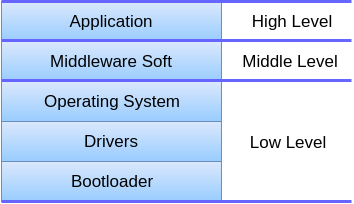
\includegraphics[width=8cm]{intro_soft_layers.png}
\note{
Перечень возможны работ связанных с разработкой программного обеспечения на базе Linux можно разделить на 3 уровня
\begin{itemize}
\item \textcolor{blue}{Low Level} - характеризует работы на уровне ядра. Сюда входят задачи Bring-up, разработка драйверов, правка на уровне ядра, закрузчика. Другими словами все что связано с работой системы вне user-space
\item \textcolor{blue}{Middle Level} - сюда входят обычно задачи по портированию библиотек стороннего программного обеспечения, настройка запуска сервисов (веб-сервера, SSH, и т.д.). Сборка и настройка базового образа прошивки, 
\item \textcolor{blue}{High Level} - уровень затрагивает разработку приложений, которые уже мало зависят от аппаратной платформы. Сюда можно отнести всякого рода UI, представленный в виде веб-интерфейса или графического(на QML и т.д). Либо можно рассмотреть то программное обеспечение которое использует библиотеки или другие средства с уровня <<Middle>>
 \end{itemize}
Каждый из уровней разработку подразумевает разный перечень компетенций от инженера. Никто не говорит, что это разделение жесткое. Вполне себе может быть инженер - который может разрабатывать ПО на всех уровнях, либо на двух близ-лежащих.
И все же давайте рассмотрим этот перечень компетенций по уровням.\\

} %note
\end{frame}

\begin{frame}[fragile]{Уровни разработки ПО во ВС}
\textcolor{blue}{Low Level} требует наличие навыков от инженера:
\begin{itemize}
\item умение читать схему электрическую принципиальную. Уверенно читать даташиты на компоненты и полученную информацию сопоставлять с исходным кодом ядра Linux.
\item понимание архитектуры ядра Linux, этапов загрузки системы на конкретном SoC
\item разработка модулей ядра, отладка на уровне ядра
\end{itemize}
\note{
Сложность работ в основном связана с тем, что инженеру необходимо хорошее понимание железа. И хороший бэкграунд знания по ядру Linux. Так как в большинстве случаев инженеру предстоит "оживить" устройство. Позволить устройству сделать свой первый вдох. \\
Моими глазами, это один из самых сложных уровней разработки ПО в проекте. И это должно нравиться инженеру. Так как, порой, приходится неделю читать мануалы, еще неделю пересматривать исходники, чтобы потом обнаружить, что в одном регистре не тот "битик" выставил. Поэтому на этом уровне остаются те, кому такой уровень действительно нравится.\\

Но на этом уровне есть один плюс ;). Я уверен что вы хоть раз в жизни да встречали программиста, читая код которого вас не покидала мысля прибить автора. Все сделано не по феншую, фиг разберешься. Но как ни странно - работает. 
Вместо того, чтобы лишать беднягу жизни - предложите ему перебраться на уровень ядра. Связано это с тем, что в большинстве случаев, код который пилится для очередного проекта, жестко привязан к железу. Поэтому ситуация использования повторного кода на другом железе - она конечно может быть. Но в редких случаях.
Поэтому на уровне ядра в большинстве случаев, если код работает - прекрасно. Рефакторинг подождет. Особенно если не предстоит расшаривать исходники. Или вы не являетесь майнтейнером. \\
З.Ы. Степень допустимой "кривости" кода в ядре конечно преувеличена. Но такое может быть на самом деле. 
\\
} %note
\end{frame}

\begin{frame}[fragile]{Уровни разработки ПО во ВС}
\textcolor{blue}{Middle Level} требует наличие навыков системного программиста и админа. А именно:
\begin{itemize}
\item Понимание принципа создания дистрибутивов ВС, их настройки в контексте запуска, 
\item Административные задачи: поднятие сервисов, их конфигурирование.
\item Ориентироваться в вопросах обеспечения безопасности Linux
\item Уметь портировать сторонние библиотеки, приложения под целевую платформу
\item Разработка демонов, библиотек взаимодействующих с BSP, ядром. 
\end{itemize}
\note{
На данном уровне как вы видите с одной стороны нужно хорошо разбираться в администрировании Linux. И при этом иметь хорошие навыки системного программиста под Linux. Больше в принципе добавить нечего\\

} %note
\end{frame}


\begin{frame}[fragile]{Уровни разработки ПО во ВС}
\textcolor{blue}{High Level} Не отличается особо от разработки ПО под компьютеры общего назначения.\\
Есть специфика, но в целом, ПО этого уровня очень далеко от "железа". 
\note{
По большому счету если взять инженера-программиста имеющего хорошие навыки в программировании приложений прикладного уровня - он справиться с задачами на данном уровне ПО. На этом уровне как раз-таки важны уже умение разрабатывать ПО, которое может использоваться на разных платформах, расширяться и т.д.\\
И если касаться встраиваемых систем. То самой сложной задачей именно по работе с железом, которую придется решить программисту - это разобраться как собранное ПО должно попасть на устройство. Утрируя конечно.\\
Например если взять тот же фреймворк QT. То можно спокойно разработать большую часть интерфейса, запуская на эмуляторе или на хост-машине. И потом уже, при необходимости, пересобрать под целевую платформу для окончательного запуска. Или нормальной ситуацией являете приглашение в команду внешнего программиста веб-разработчика. Если стоит задача разработать веб-интерфейс.\\

} %note
\end{frame}

\section{Закрепление рассмотренного в рамках проекта <<ОКО>>}
\begin{frame}[fragile]{Уровни ПО}
Рассмотрим на примере следующей задачи. \\
Сделать поддержку управления: 
\begin{itemize}
\item инфракрасной подсветкой для включения в ночное время.
\item управление <<сухим контактом>>, который в свою очередь может подавать управляющие команды на другую аппаратную подсистему путем изменения своего состояния <<замкнут/разомкнут>> 
\end{itemize}
\note{
Давайте не уходя далеко начнем с уровней ПО. Представим, что нам уже предстоит спроектировать управление ИК-подсветкой и реле. При этом, условно говоря, мы знаем как это реализовано на аппаратном уровне. У нас есть навыки разработки ПО на уровне ядра Linux. 
Как это может быть сделано аппаратно на реальном устройстве - вдаваться не будем. Примем, что нам известно как управлять программно из ядра.
И мы можем выполнить поставленные задачи.\\

} %note
\end{frame}



\begin{frame}[fragile]{Уровни ПО. Управление ИК-подсветкой}
Задача с ИК-подсветкой сводиться к решению <<послать>> команду аппаратной части включить ее или выключить. \\
Кто будет принимать решение о управление оставим за рамками примера. Поэтому нужно реализовать поддержку следующих управляющих команд:
\begin{itemize}
\item Включить - фактически замкнуть цепь питания ИК-подсветки
\item Выключить - разомкнуть 
\end{itemize}

\end{frame}

\begin{frame}[fragile]{Уровни ПО. Управление <<Сухим контактом>>}
Сухой контакт может иметь состояния - <<рабочее>> и <<нерабочее>>. И с точки зрения электрической цепи в нерабочем/пассивном состоянии может быть вида: 
\begin{itemize}
\item \textcolor{blue}{Нормально разомкнутый} - в нерабочем состоянии - цепь разомкнута, в рабочем - цепь замкнута
\item \textcolor{blue}{Нормально замкнутый} - обратное предыдущем
\end{itemize}
\note{
Работая с реле, кнопками и т.д. вводятся понятия, которые характеризуют его рабочее и нерабочие состояния. Так обычная кнопка является нормально разомкнутым видом контакта. Так как она замыкает цепь при нажатии, размыкает- при отпускании. \\
Исходим из того, что мы на этапе проектирования не можем с уверенностью сказать, что для <<клиента>> сухого контакта будет рабочим состоянием - когда мы замкнем реле, или разомкнем. Поэтому мы должны сделать поддержку настройки рабочего состояния. А конечный пользователь уже будет решать какой вид контакта задать в камере. \\
} %note
\end{frame}

\begin{frame}[fragile]{Уровни ПО. Управление <<Сухим контактом>>}
Сухой контакт может быть еще двух режимов работы:
\begin{itemize}
\item \textcolor{blue}{Bistable} - может свободно переключаться между состояниями
\item \textcolor{blue}{Monostable} - после установки в рабочее состояние, контакт возвращается в нерабочее через определенный интервал времени. Это время может настраиваться  
\end{itemize}
\note{
Само поведение контакта тоже может задаваться пользователем. В случае с Monostable режима пользователь может задать интервал возвращения в нерабочее состояние. Например 3 секунды.\\

}%note
\end{frame}


\begin{frame}[fragile]{Уровни ПО. Упрощенная схема управления}
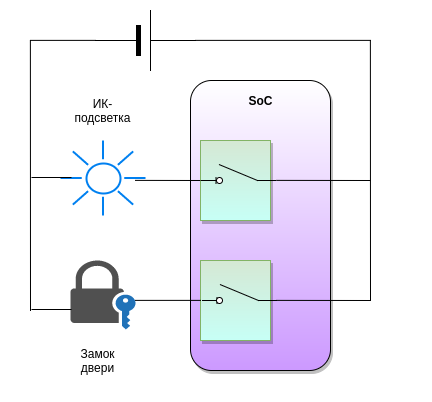
\includegraphics[height=5cm]{contacts.png}
\note{
Вам может показаться, что сухой контакт, имея такое поведение имеет более сложную реализацию на аппаратном уровне. По сравнению с ИК-подсветкой. Но это не так.\\
 На самом деле с точки зрения аппаратных интерфейсов обе задачи решаются одинаково - управление происходит через порты GPIO (будет далее по лекциям). \\
 
Очень уж условно и символично представлена схема подключения. Представим что сухой контакт у нас управляет неким замком двери. Либо чем-то другим, что подключит к нему пользователь камеры. 
В прямоугольниках зеленоватого цвета у нас отражена некая аппаратная реализация управления цепью. И получается, мы знаем как замыкать/размыкать эти ключи. И при замыкании цепи питание идет на подсветку и замок.  \\
}%note
\end{frame}


\begin{frame}[fragile]{Уровни ПО. Low Level}
Инженер реализует драйвер, который:
\begin{itemize}
\item Создает два файла-устройства в каталоге /dev. Которые являются символьными устройствами. То есть поддерживают операции 'Open', 'Write', 'Read', 'Close'
\item Файлам-устройств даются имена /dev/port1 и /dev/port2 
\item Чтобы замкнуть цепь, достаточно открыть файл и послать строку с '1', разомкнуть - послать '0'
\item Для чтения состояния цепи - выполнить операцию чтения. Вернет строку с '1' - замкнута, '0' - разомкнута
\end{itemize}
\end{frame}
\note{
Первым за работу берется условно Low Level инженер. Посмотрев схему, он видит, что по сути с точки зрения SoC-a, что управление подсветкой, что управление сухим контактом. Одна и та же задача. Поэтому не долго думая. Он реализует драйвер. В котором твориться магия, но с точки зрения user-space мы видим два файла устройства. С которыми мы можем работать как с обычными файлами. Реализовав этот драйвер инженер перевел задачу выше на уровень с описанием принципа работы. И добавим заметку:
\begin{itemize}
\item файл /dev/port1 управляет подсветкой
\item файл /dev/port2 - сухим контактом
\item Запишешь символ '1' - замкнуться цепи
\item Запишешь символ '0' - разомкнем цепи
\item Исходное состояние на этапе старта устройства - '0'
\end{itemize} 
}%note
\end{frame}


\begin{frame}[fragile]{Уровни ПО. Middle Level}
Инженер реализует динамическую библиотеку, которая имеет API (основные):
\begin{itemize}
\item OpenRelayOutput(devname) - возвращает файловый дескриптор устройства
\item CloseRelayOutput(devfd)
\item SetRelayOutputSettings(devfd, settings),
\item GetRelayOutputSettings(devfd, *settings)
\item SetRelayOutputState(devfd, enable),
\item GetRelayOutputState(devfd, *enable),
\end{itemize}
\note{
Инженер, почитав спецификацию по управлению, и то, что ему предоставил инженер Low Level решил следующее:
\begin{itemize}
\item я не вижу архитектурной разницы между принципами работы с подсветкой и контактом.
\item есть только бизнес-правило для ИК-подсветки. Она может иметь только Bistable режим. Поэтому разделять между собой ИК-управление и сухим контактом в рамках библиотеки не буду.
\item сегодня ИК-подсветка весит на устройстве /dev/port1, а завтра может передумают и поменяют порты. Поэтому к файлам устройств привязываться не буду на уровне библиотеки.
\end{itemize}
И в итоге реализует динамическую библиотеку. Которая с точки зрения API представляет:
\begin{itemize}
\item <<Открытие>> контакта по имени устройства. Возвращает файл открытого дескриптора
\item Инициализацию настроек порта через функцию \textcolor{blue}{SetRelayOutputSettings()}. где \textcolor{blue}{settings} представляет собой структуру, в которой указываются параметры: режим Bistable/Monostable, нерабочее состояние, время возвращения в нерабочий режим в режиме Monostable. И естественно поддержка считывания настроек.
\item Установка требуемого состояния с помощью \textcolor{blue}{SetRelayOutputState}, где \textcolor{blue}{enable} - True если задаем рабочий режим.
\end{itemize}
Всю магию, связанную с поддержкой режимов работы порта он скрывает внутри библиотеки. Так что работая с этой библиотекой скрывается то, что по факту библиотека будет слать то '1' то '0'.\\
Реализовав это инженер передает инициативу на верх с предоставленным API. И информацией. Что для управления подсветкой юзать /dev/port1, контактом - /dev/port2.\\

}%note
\end{frame}


\begin{frame}[fragile]{Уровни ПО. High Level}
Инженер принимает решение разработать:
\begin{itemize}
\item демона \textcolor{blue}{InfraLightDaemon} - управление подсветкой
\item демона \textcolor{blue}{RelayOutputDaemon} - управление реле
\item Через определенные IPC демоны будут получать инструкции по управлению от других подсистем.
\end{itemize}

\note{
Программист разрабатывает два демона по управлению. Каждый демон: 
\begin{itemize}
\item знает с каким устройством /dev/portX работать. Это может быть жестко прописано в исходниках. либо может передаваться через аргументы командной строки или переменные окружения
\item знает как должен настраиваться порт. Так в InfraLightDaemon будет явно настраиваться порт на Bistable режим. А в демоне RelayOutputDaemon должна быть реализована поддержка изменения настроек. Например через веб интерфейс меняется режим работы сухого контакта с Bistable на Monostable - демон должен подхватывать и применять
\item Демоны будут получать от разных подсистем инструкции по управлению. Как это будет происходить оставим за рамками примера.
\end{itemize}

И как мы видим с точки зрения самого управления класс задач кажется совсем простой. По сути дергай только API библиотеки.\\
Но как и говорилось ранее, на этом уровне приходиться решать задачи возможного расширения и масштабируемости. Так инженер должен учитывать то, что сегодня он собирает прошивку для конкретной модели устройства, но завтра, этих моделей будет три. И те же порты могут быть поменяны. В одной модели будут одни источники управления демонами, в другом - другие. А может определенная модель камеры будет иметь один порт. На который может быть нахлобучена либо подсветка, либо сухой контакт. В общем, смысл вы, я думаю, поняли.\\
}%note
\end{frame}


\begin{frame}[fragile]{Определяемся с аппаратной частью для проекта OKO}
Для реализации проекта IP-камеры мы рассмотрим следующие SoC-и:
\begin{itemize}
\item Hi3516A - SoC от HiSilicon. URL на SDK см. на слайде <<Ссылки>> 
\item i.MX6Solo -SoC от NXP/Freescale. URL там же 
\item Raspberry PI3 c SoC BCM2837. Broadcom производитель
\end{itemize}
\note{
Для дальнейшего изложения материала уже имеет смысл определяться с железом. На базе чего будем делать камеру. Остановились на решениях, которые представлены на слайде. Выбор первых двух чипов был обусловлен доступностью SDK. Которая позволит и дальше пояснять материал ссылаясь на конкретные примеры. RPI3 было решено включить так как в основе тренинга лежит данная модель. \\
Сам доступ к отладочным платам у нас если и может быть, то только к RPI3. В рамках лекций и не планировалось что либо запускать. Поэтому достаточно будет обзорной части.\\


}%note
\end{frame}


\begin{frame}[fragile]{SoC. Hi3516A}
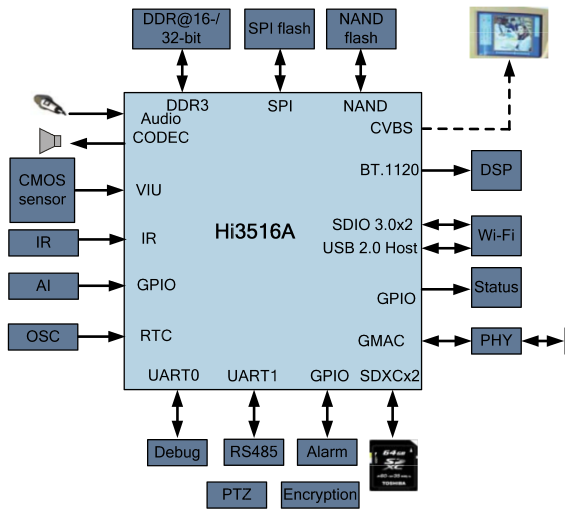
\includegraphics[height=6.5cm]{Hi3516A.png}
\note{
Если вы скачали SDK по ссылке и распаковали, то вы сможете открыть документ\textcolor{blue}{ Hi3516A/Hi3516D HD IP Camera SoC Data Sheet.pdf}  в каталоге\textcolor{blue}{ <SDK PATH>/00.hardware/chip/document\_en/}. Исходя из названия вы уже поняли, что это даташит на SoC-и. Документ совсем не большой. В 6 страниц всего. Он краткий, для первичного осмотра характеристик камней. Но рядом уже лежат развернутые даташиты с полным описанием.  
Представлен рисунок с 6-й страницы даташита, который показывает его возможности.\\
Если, увидев данных рисунок, вы сказали "М-м-м-м. Какой вкусный камушек..." и в восторге задрыгали ножками - вы определенно эмбеддер. Сразу приходит в голову, что чип явно заточен под системы видеонаблюдения, так как в нем есть все что нам нужно, и даже больше:
 \begin{itemize}
\item VIU (Video Input Unit) - для захвата видео-данных с аналогового камеры
\item Audio Codec - для захвата звука и с кодированием на лету. 
\item GPIO - для управления инфракрасной подсветкой и сухим контактом
\item GMAC - Еthernet-подключение с поддержкой POE (Power over Ethernet)
\item Поддержка карты памяти
\item Можно подключить еще Wi-Fi чере USB или SDIO
\end{itemize}
А кроме этого, мы еще можем задействовать возможности для:
 \begin{itemize}
\item Реализации управления поворотным устройством камеры (PTZ)
\item Послать видеоданные через BT.1120 на какую-нить FPGA или DSP-процессор. Которые будут заниматься анализом видео (детекторы и т.д.)
\item Сразу послать видео на дисплей через композитный выход (CVBS)
\item Есть аппаратная поддержка шифрования данных. Возможность организации секьюрности - это хорошо.
\end{itemize}
Не знаю как вы, но я в экстазе. А давайте, продлим наше удовольствие и заглянем еще и под капот чипа.\\

} %note
}%note
\end{frame}

\begin{frame}[fragile]{SoC. Hi3516A}
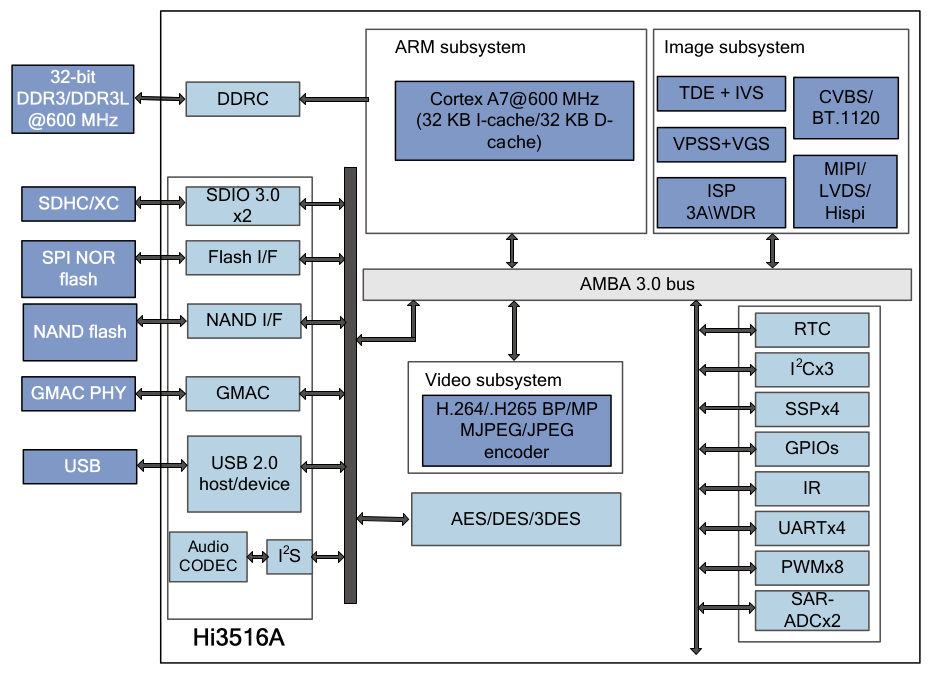
\includegraphics[height=6.5cm]{Hi3516A_block.png}
\note{
Рисунок на слайде представлен с того же документа. Сама детализация подробно описана с сопутствующим текстом. Выжимки из которой я и приведу. 
\begin{itemize}
\item Крутится у нас все на Arm-процессоре
\item На лету может кодировать аппаратно видео:
  \begin{itemize}
  \item сразу 3 потока: 1080p@30fps + 720p@30fps + VGA@30fps\\
  (где 1080p@30fps это 1920x1080 разрешение; полный кадр не черезстрочный; 30 кадр/сек.) 
  \item или 2: 1080p@60 fps + VGA@30fps
  \item или 2: 5-megapixel@30fps + VGA@30fps 
 \end{itemize}
\item Может накладывать поверх видео графику (текст и т.д.)
\item Image signal processor (ISP) - компенсация битых пикселей сенсора, шумоподавление пикселей, компенсация искривления оптической линзой, и другие важные моменты, которые существенны для систем видеонаблюдения.
\item Аппаратное кодирование звука в кодеки, характерные для VOIP - G.711, ADPCM и т.д. 
\item Периферия, стандартная. Все что нужно есть.
\end{itemize}
Очень удачный чип, полностью подходит под наши задачи.
}%note
\end{frame}


\begin{frame}[fragile]{SoC. i.MX6Solo}
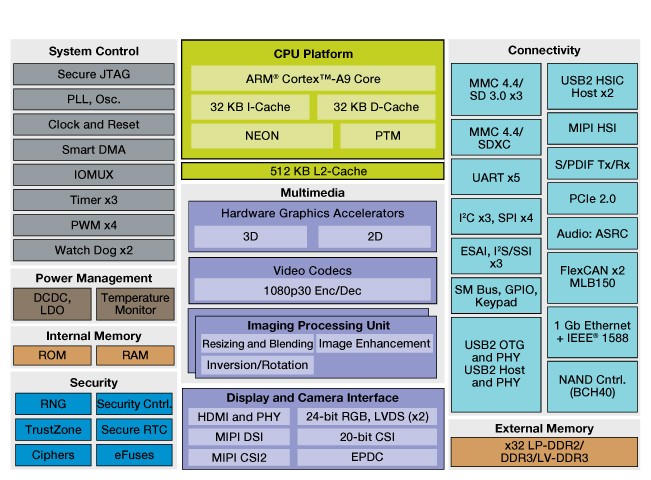
\includegraphics[height=6.5cm]{IMX6S_block.png}
\note{
Изучать SoC i.MX6Solo мы начнем сразу с блок схемы. Если сравнивать с предыдущим SoC-ом, то сразу можно отметить, что данный чип является более универсальным решением, которые ориентирован на мультимедиа устройства. Это могут быть мультимедиа решения для авто, проигрывание запись аудио и звука, планшето-подобные решения и т.д. Для нашего проекта он также может быть рассмотрен, так как есть подходящие характеристики:
\begin{itemize}
\item Есть, прежде всего, подсистема кодирования и декодирования видео (обратите внимание что в HiSi-чипе было только кодирование
\item Есть подсистема наложения графики причем и 3D
\item Есть интерфейсы MIPI CSIx для захвата сырых данных видео
\item С периферией также все в порядке.
\item Но обращаем внимание, что по сравнению с HiSi-чипом:
 \begin{itemize}
   \item Есть подсистема кодирования и декодирования видео (обратите внимание что в HiSi-чипе было только кодирование
   \item Есть подсистема наложения графики причем и 3D
   \item Есть интерфейсы MIPI CSIx для захвата сырых данных видео
   \item С периферией также все в порядке.
 \end{itemize}
\end{itemize}

И, я думаю, у вас закралась мысль "А не слишком ли чип наворочен для нашего проекта", если сравнивать с предыдущим вариантом. Я соглашусь. Он избыточен, если стоит задача чисто захватить данные, сжать и пустить в сеть или захватить. Еще и ARM-процессор мощнее будет. Но давайте себе представим, что мы не ущемлены в средствах и нас абсолютно не интересует себестоимость разработки. \\
}%note
\end{frame}


%--------- template
\begin{frame}[fragile]{SoC. BCM2837  }
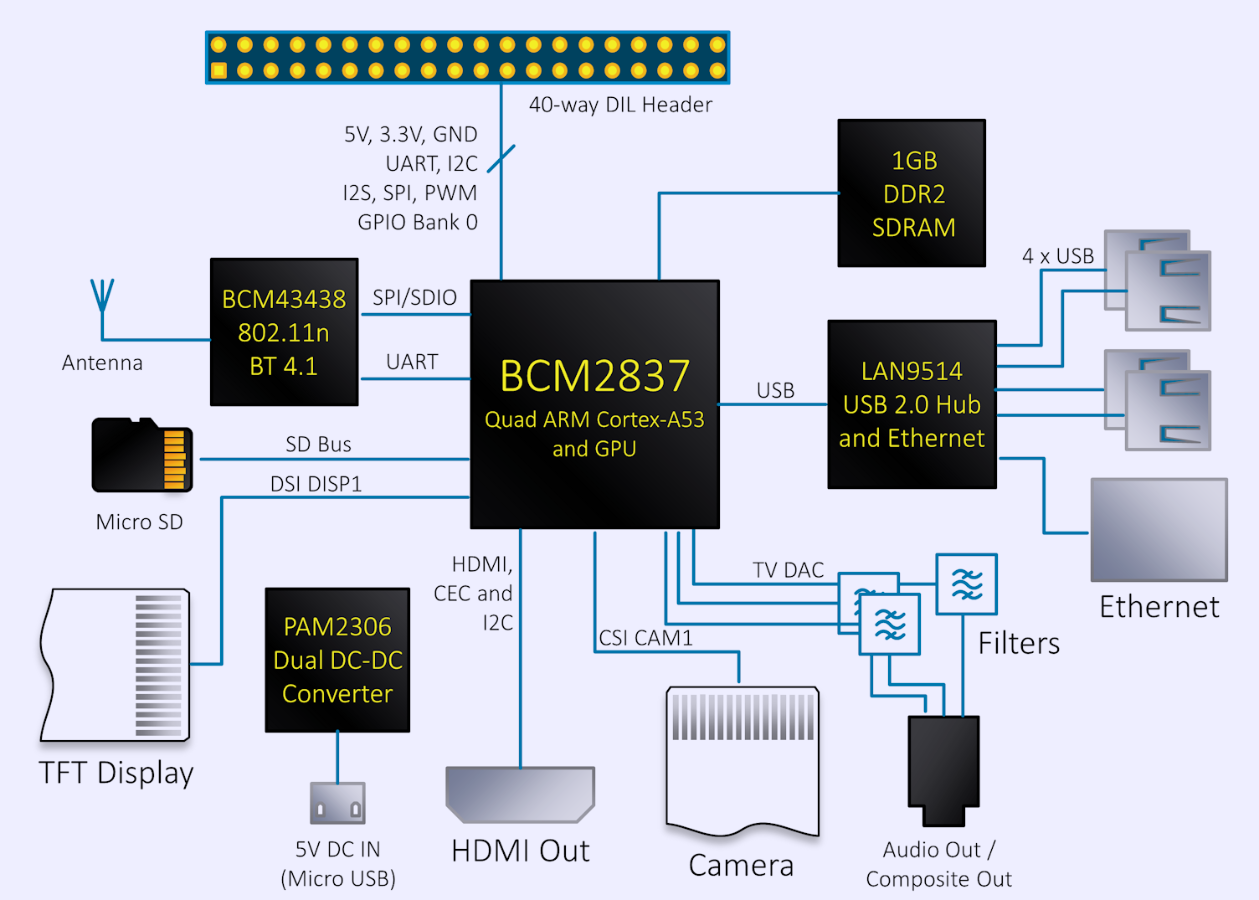
\includegraphics[height=6.5cm]{RPI3_block.png}\\
Источник \url{https://xdevs.com/article/rpi3_oc/}
\note{
На BCM2837 вы не сможете найти публичный официальный даташит. Можно найти из отдельных источников описание начинки. Либо найти даташит на более ранний чип BCM2835, на который идет отсыл вида "Все примерно так-же но есть отличия". Оно и понятно, Raspberry PI3 рассматривается как однопалатный мультимедиа компьютер. То есть как законченный продукт.  Для него полностью реализована поддержка на стороне ядра Linux. И вся периферия.\\
 Можно отметить следующие характеристики с официального сайта: 
\begin{itemize}
\item 64 битный Arm-процессор
\item Есть GPU
\item Есть CSI-порт для камеры
\item Aппаратная поддержка H.264,MJPEG отсутствует. То есть придется программно сжимать видео в нашем проекте.
\item Аудиовхода вообще нет. Вот нам не везет. Придется юзать USB-звуковую карту. Ну или камера будет глухой.
\item Периферия, в плане портов - достаточно для нашего проекта. 
\end{itemize}
Получается, что если сравнивать с другими нашими чипами, то этот вариант может выигрывать только за счет того, что уже реализована плата, и не нужно делать обвязку. И процессор мощнее чем у других. Но в рамках нашего проекта все задачи придется выполнять программно. А где-то еще и придумывать костыли. \\
И возвращаясь к утверждению, что \\
\textcolor{blue}{<<иногда приходиться решать, на каком уровне будет реализована задача - аппаратном или программном>>}\\
Мы видим, что так и есть. поддержку сжатия в H.264 мы можем сделать аппаратно заюзав первых два чипа. Либо сделать программно. Но на RPI3 мы врятли добьемся кодирования с характеристиками 60 fps в fullHD,  как это нам позволяет сделать чип от Hi-Si.\\

} %note
\end{frame}

\begin{frame}[fragile]{Процессоры ARM}
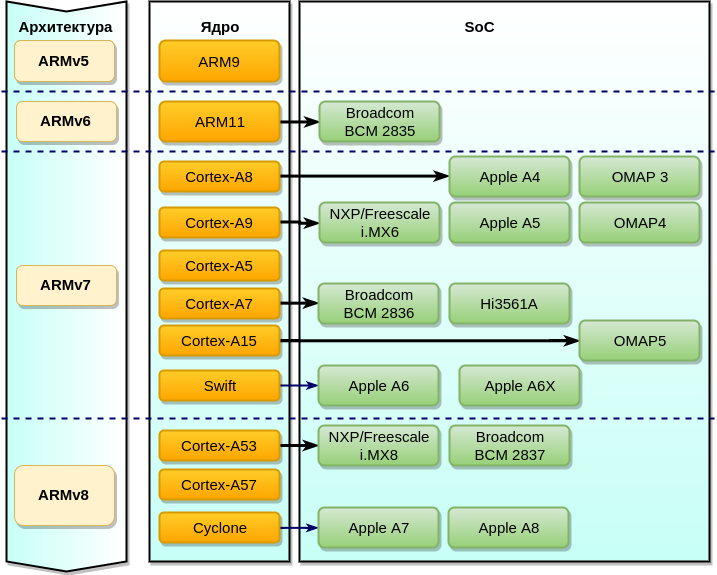
\includegraphics[height=6.5cm]{arm_family.png}\\
Самостоятельно: Изучить процессоры семейства Cortex-M, Сortex-R, их специфику
\note{
Мы с вами рассмотрели чипы, и каждый из них сделан на базе ARM-процессора. На слайде представлены семейства процессоров ARM и примеры чипов на базе которых они сделаны. \\
Прежде всего следует отметить тот момент, что порой можно запутаться между понятиями \textcolor{blue}{<<Семейство>>}, \textcolor{blue}{<<Архитектура>>}, \textcolor{blue}{<<Ядро>>}. И применять их неправильно в нужном контексте. Поэтому я позволю себе еще раз пояснить ссылаясь на данный рисунок.\\
Компания ARM Holdings (далее ARMH) является проектировщиком архитектуры RISC-процессоров. Она не изготовляет процессоры как таково, а продает лицензии другим компаниям-производителям.  ARM-архитектура подразумевает фактически набор команд ARM, которые могут выполняться на конечном ядре процессора. И эти наборы команд и подразумеваются под \textcolor{blue}{версией архитектуры} ARM. На рисунке я показал только часть версий, начиная с ARMv5 до ARMv8. И еще и сгруппировав. Но есть и более ранние версии. Некоторые уже считаются устаревшими, но некоторые используются в микроконтроллерах.\\
Помимо архитектуры ARMH еще проектирует и \textcolor{blue}{ядра процессоров}. Опять же, она их не изготовляет, а только продает лицензию на изготовление. Так, например, ARMH спроектировала ядро процессора ARM11. Лицензию на это ядро процессора купила компания Broadcom и на базе его сделала SoC BCM2835. И уже на базе этого SoC-a выпустила одноплатный компьютер Raspberry PI первой версии. \\
Несколько ядер, в рамках одной архитектуры объединяются в \textcolor{blue}{семейства}. Так в одно семейство Cortex-A объеденены ядра с архитектурой ARMv8. А ядра Cortex-A53, Cortex-A57 уже объеденены в семейство Cortex-A50\\
Но есть еще производители, которые изготавливают собственные ARM ядра. Например компания Apple. Которая первая версии своих SoC-в делала покупая лицензии на ядра ARM семейства Cortex-A. А потом уже начала выпускать свои ядра - Swift, Cyclone. \\
Ну вот примерно так все выглядит. \\
На более детальную информацию даны источники на слайде <<Ссылки>>
} %note
\end{frame}

\section{Варианты взаимодействия с устройством}
\begin{frame}[fragile]{Отладочный порт}
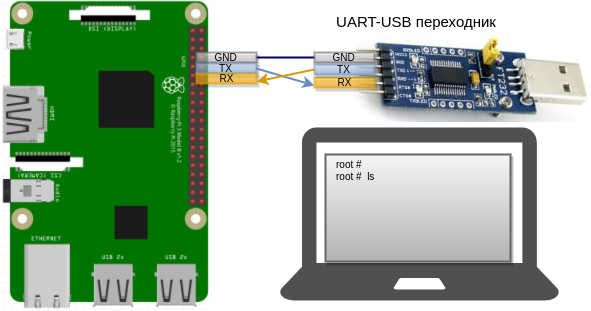
\includegraphics[height=6cm]{conuart.png}
\note{
Пристуив к разработке прошивки для устройства нам необходимо, прежде всего, наладить общение с устройством. Самой распространенным вариантом получить доступ к устройству является доступ через UART-порт. Сам интерфейс будет рассмотрен в других лекциях. При загрузки операционной системы Linux на уровне загрузчика и самого ядра прописывается, что все сообщения загрузки посылать в определенный UART-порт. И при необходимости вы можете:\\
\begin{itemize}
\item увидеть лог загрузки устройства
\item скачивать и заливать файлы. Пусть это и будет самая медленная операция по сравнению с другими вариантами
\item выполнять задачи (подправить конфиги, удалить файлы, отправить на перезагрузку устройство)
\end{itemize}
Для получения доступа к устройству с компьютера используется специальный UART-USB или UART-COM конвертер. Для его подключения достаточно задействовать 3 выхода:
\begin{itemize}
\item GND - земля. 
\item TX - передача данных
\item RX - прием данных
\end{itemize}
Обратите внимание, что на рисунке между устройством и переходником пины RX, TX подключены не напрямую. Что логично. Одна сторона передает, другая принимает.\\
Когда вы подключаете конвертер к компьютеры - появляется файл устройства /dev/ttyUSBx. Через этот файл устройства вы будете общаться с устройством.  \\
Для общения необходимо запустить программу-терминал. Программа-терминал по сути является мостом, который позволяет увязать консоль устройства с консолью PC через отладочный порт. Как настраивать программу-терминал будет рассмотрено на других лекциях. \\
Основной плюс данного способа в том, что он позволяет отследить логи загрузки с самого начала. Либо еще сделать первичную прошивку устройства

} %note
\end{frame}

\begin{frame}[fragile]{Сеть}
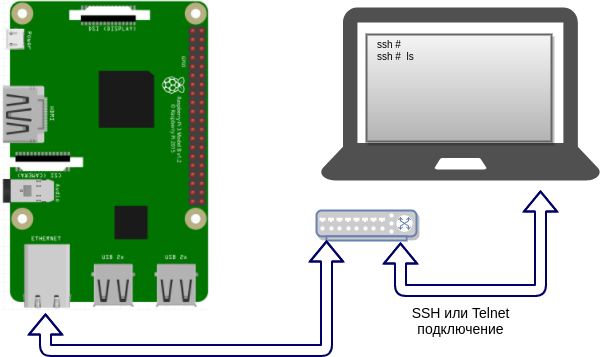
\includegraphics[height=6cm]{conethernet.png}
\note{
Работа через отладочный порт неудобна в случае, если:
\begin{itemize}
\item стоят часто задачи залить, скачать файлы
\item устройство находится удаленно от хоста
\end{itemize}
В случае, если у устройства есть сетевые интерфейсы - вы можете поднять SSH или Telnet сервисы. Используя которые вы получите удаленный доступ. Скорость обмена данными возрастет, но доступ к самому устройству будет только после того, как устройство загрузится и поднимет сеть. \\
Естественно, если есть желание можно поднять и FTP. Но обычно в этом нет необходимости, так как именно для обмена файлами удобнее использовать сетевую файловую систему\\

} %note
\end{frame}

\begin{frame}[fragile]{NFS}
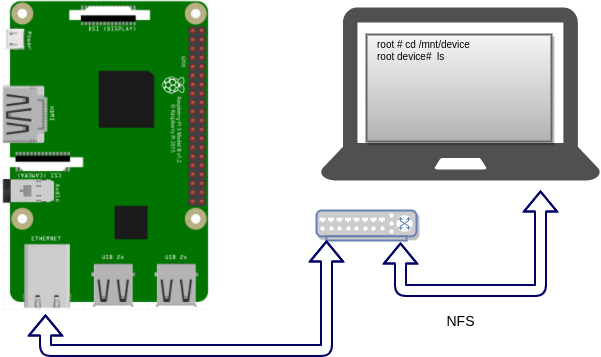
\includegraphics[height=6cm]{connfs.png}
\note{
Для обмена данных между устройством и хостом можно поднять сетевую файловую систему. Обычно алгоритм такой:\\
\begin{itemize}
\item на хосте вы запускете NFS-сервер. И расшариваете определенную папку. Например /home/user/dev/nfs/ 
\item на устройстве монтируете удаленную папку. Например в /mnt/host
\item для передачи файла достаточно копировать его в заданные каталоги
\end{itemize}
Можно выполнить операцию и наоборот. Серверной частью будет выступать устройство.\\

} %note
\end{frame}

\begin{frame}[fragile]{Загрузка устройства по сети}
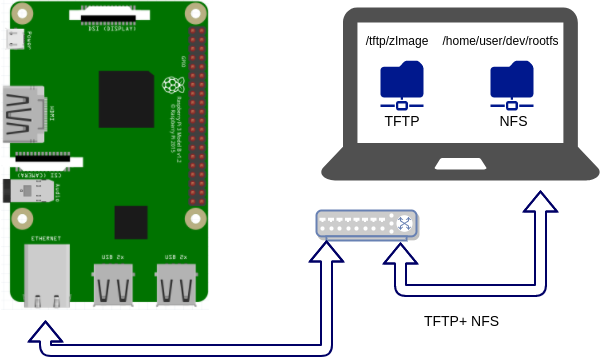
\includegraphics[height=6cm]{conboot.png}
\note{
Опять же используются возможности сети. В данном случае мы можем настроить устройство так, что оно будет загружать ядро Linux по сети, и корневую файловую систему также будет монтировать по сети. 
Алгоритм может быть таким:
\begin{itemize}
\item На хосте поднимаем TFTP-сервер (облегченная версия FTP-сервиса). 
\item Создаем каталог /tftp/ куда копируем ядро Linux
\item Корневую файловую систему устройства расшариваем в виде папки по NFS пусть будет /home/user/dev/rootfs/
\item Загрузчик устройства настраиваем так, чтобы он:
\begin{itemize}
\item поднимал сетевое подключение на устройстве
\item скачивал ядро Linux по сети
\item Передавал управление ядру Linux и указав в параметрах, что корневая файловая система может быть получена по NFS
\item Устройство загружается, фактически, используя ресурсы на хосте
\end{itemize}
\end{itemize} 
Такой вариант наиболее часто используется на ранних этапах проекта. Когда необходимо очень часто перепрошивать устройство, чтобы увидеть результат. Этот способ позволяет операцию разработки значительно ускорить.\\

Более подробно эти моменты будут рассмотрены в других лекциях, либо на практике. \\

} %note
\end{frame}

\begin{frame}[fragile]{JTAG}
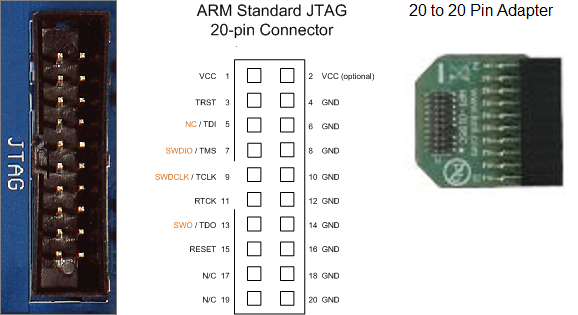
\includegraphics[height=6.5cm]{conjtag.png}\\
Источник \url{http://www.keil.com/support/man/docs/ulinkpro/ulinkpro_cs_connectors.htm}
\note{Еще один способ наладить общение с устройством, это задействовать JTAG-интерфейс.\\
Этот интерфейс предназначен в большей степени для аппаратного тестирования, отладки. Через него можно проверить именно корректность работы аппаратной части, а не софтверной. \\
Но иногда приходиться с ним иметь дело, когда после вашего колдовства устройство превращается в <<кирпич>>. То есть не подает никаких признаков жизни.\\
Всегда через JTAG-интерфейс можно зашить прошивку во внутреннюю память устройства. Либо считать ее.\\

} %note
\end{frame}


\section{Яыки программирования}
\begin{frame}[fragile]{Основные языки для разработки}
\begin{itemize}
\item Си
\item C++
\item Bash
\end{itemize}
\note{
Лидирующие позиции занимает язык Си. Связано это с тем, что разработку драйверов ядра Linux приходится вести на языке Си. Вендоры часто предоставляют BSP также на языке Си. В принципе язык Си используется на всех уровнях разработки ПО\\
Язык С++ используется в основном на уровне Middle и Hight уровней\\
Bash - используется для разработки скриптов. 
} %note
\end{frame}

\begin{frame}[fragile]{Другие}
\begin{itemize}
\item Lua
\item Java
\item JavaScript
\item Rust
\end{itemize}
\note{
Другие языки, которые также могут быть использованы это:
\begin{itemize}
\item Lua - легковесный, интерпретируемый язык. Может взаимодействовать с Си-библиотеками.
\item Java - если рассматривать в контексте разработки под Android
\item JavaScript - при разработке веб-интерфейса
\item Rust - последнее время все чаще про него приходится слышать в embedded-области. И потиху начинает отжимать позиции у языка Си благодаря своим преимуществам.
\end{itemize}
} %note
\end{frame}


\section{Справочные материалы}
\begin{frame}[fragile]{Ссылки}
\begin{itemize}
\item Hi3516A SDK: \\
\url{https://sourceforge.net/projects/hisi/files/SDK/Hi3516/} 
\item i.MX6Solo SDK: \\
\url{https://www.nxp.com/support/developer-resources/run-time-software/i.mx-developer-resources/i.mx-6-i.mx-7-i.mx-8-series-software-and-development-tool-resources:IMX_SW}
\item Процессоры ARM: особенности архитектуры, отличия и перспективы \\
\url{https://itc.ua/articles/protsessoryi-arm-osobennosti-arhitekturyi-otlichiya-i-perspektivyi/}

\end{itemize}
\end{frame}


\begin{frame}[fragile]{Ссылки}
\begin{itemize}
\item Процессоры ARM: производители и модели \\
\url{https://itc.ua/articles/protsessoryi-arm-proizvoditeli-i-modeli/}
\item Список архитектур ARM (wiki)\\
\url{https://ru.wikipedia.org/wiki/%D0%A1%D0%BF%D0%B8%D1%81%D0%BE%D0%BA_%D0%B0%D1%80%D1%85%D0%B8%D1%82%D0%B5%D0%BA%D1%82%D1%83%D1%80_ARM} 

\end{itemize}
\end{frame}


%--------- frame template 
%\section{SECTION NAME}
%\begin{frame}[fragile]{TITLE}
%text
%\note{\begin{itemize}
%\item 
%\end{itemize}
%} %note
%\end{frame}

\end{document}

